\documentclass[11p,a4paper]{article}

\usepackage{booktabs}
\usepackage{authblk}
\usepackage{amsmath}
\usepackage{amsfonts}
\usepackage{amssymb}
\usepackage{amsthm}
\usepackage{mathtools}
\usepackage{mathrsfs}
\usepackage{float}
\usepackage{natbib}
\usepackage{graphicx}
\usepackage{subcaption}


\usepackage[hidelinks]{hyperref}
\usepackage{xcolor}

% Hypersetup for hyperlinks
\hypersetup{
	pdftitle={Your title here},
	pdfauthor={Your name here},
	pdfsubject={Your subject here},
	pdfkeywords={keyword1, keyword2},
	bookmarksnumbered=true,     
	bookmarksopen=true,         
	bookmarksopenlevel=1,       
	colorlinks=true,            
	pdfstartview=Fit,           
	pdfpagemode=UseOutlines,    % This is the option you were looking for
	pdfpagelayout=TwoPageRight,
	linkcolor={red!50!black},
	citecolor={blue!50!black},
	urlcolor={blue!80!black}
}

\begin{document}

\title{Sample LaTeX Document}
\author{Your Name}
\date{\today}

\maketitle

\section{Introduction}
This is a sample LaTeX document that demonstrates various features, including math equations, referencing, figures, and tables. We have used here the \texttt{hyperref} package to enable clickability.

\section{Body}
\subsection{Math}
LaTeX is great for typesetting math equations. Here's an example of an inline equation: $E = mc^2$, and here's a display equation:
\begin{equation}
    \int_{0}^{\infty} e^{-x^2} dx = \frac{\sqrt{\pi}}{2}
\end{equation}

\subsection{Referencing}
You can reference sections, equations, figures, and tables using labels and the \texttt{ref} command. For example, in Section~\ref{sec:figures}, we will see how to include figures.

\subsection{Citations}
For this Math course, we use some materials from \citet{simon1994mathematics}. The book is praised by many researchers as a must-have math book for economists \citep{sydsaeter2008further}. 

Please use package \texttt{natbib} because it is compatible with the package \texttt{hyperref}. To cite text, use \texttt{citet\{key1\}}, to cite with parenthesis, use \texttt{citep\{key2\}}. Make sure the keys match what you declared in the .bib file. 

At the end of the document, to print the reference list, use the command \texttt{\textbackslash bibliography\{bibliography.bib\}}. You can choose the style of the document by stating \texttt{\textbackslash bibliographystyle\{style\}} before printing the bib. There are many styles. Here, we use \texttt{apalike} -- the most commonly used.


\section{Figures}\label{sec:figures}
Figures can be included using the \texttt{graphicx} package. Below is an example of a figure -- the screenshot of a .bib file:

\begin{figure}[H]
    \centering
    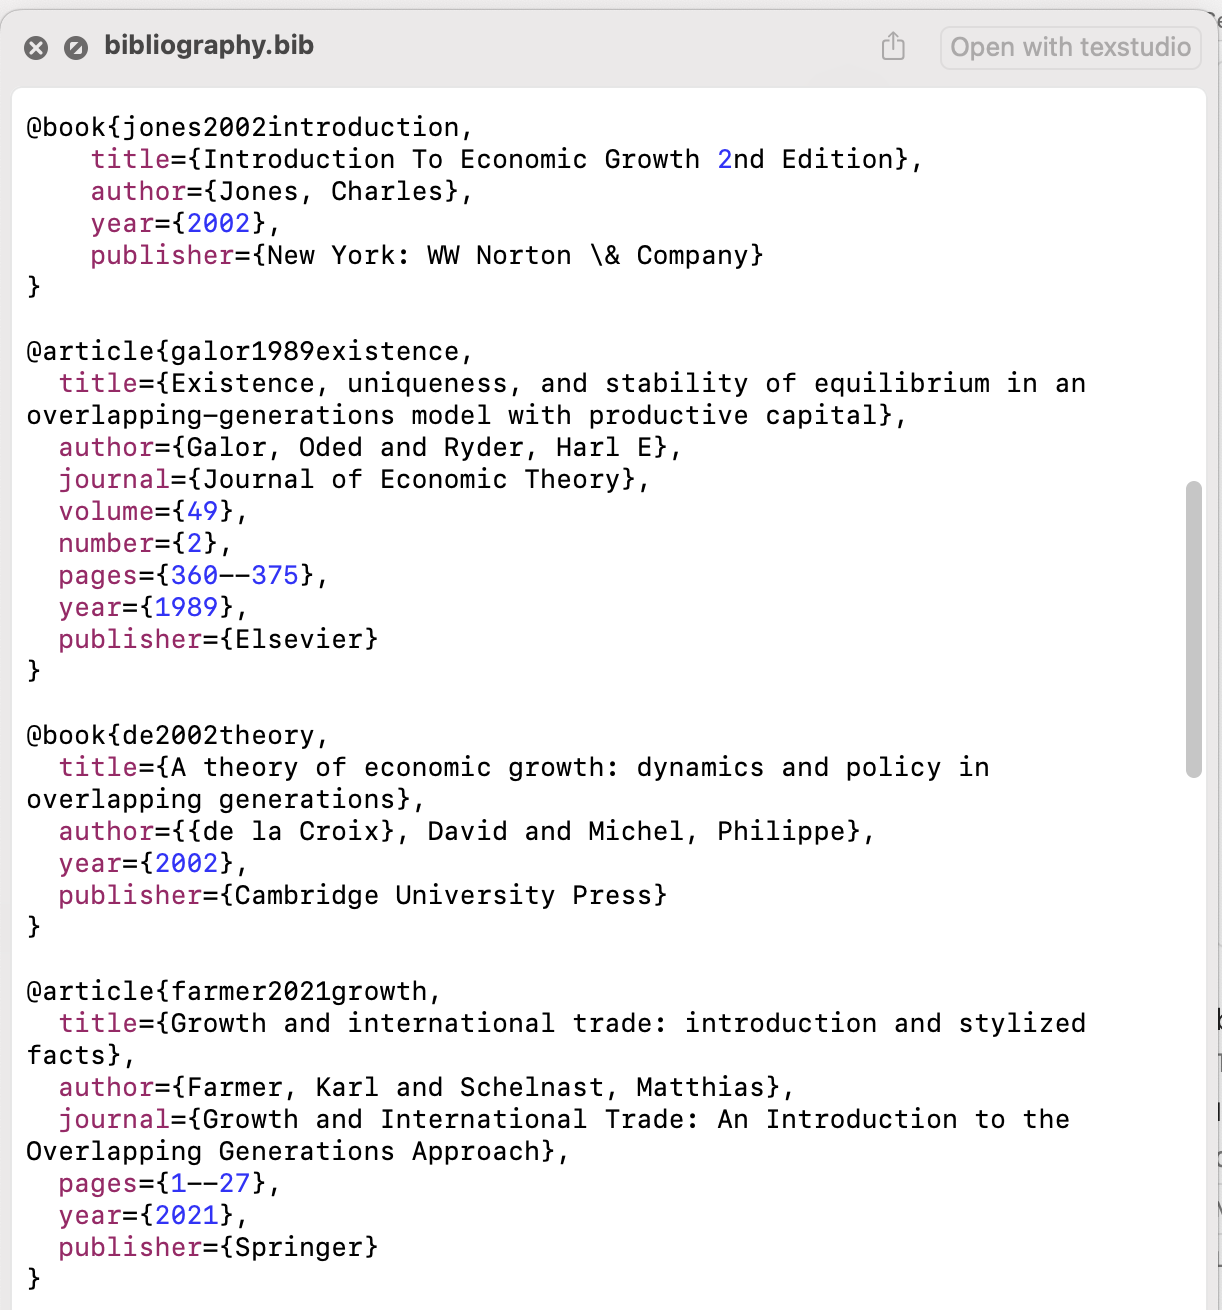
\includegraphics[width=0.6\linewidth]{bib_fig.png}
    \caption{Bibliography format}
    \label{fig:example}
\end{figure}

As shown in Figure~\ref{fig:example}, you can refer to figures by their label.

\section{Tables}
Tables can be created using the \texttt{tabular} environment. Here's an example:

\begin{table}[htb]
    \centering
    \begin{tabular}{c c}
        \hline
        Name & Age \\
        \hline
        Alice & 25 \\
        Bob & 30 \\
        Charlie & 28 \\
        \hline
    \end{tabular}
    \caption{Example table}
    \label{tab:example}
\end{table}

You can reference tables by their label, just like figures. Table~\ref{tab:example} shows an example table.

\section{Conclusion}
This concludes our sample LaTeX document. It demonstrates how to include math equations, referencing, figures, and tables. Happy LaTeXing!


\bibliographystyle{apalike}
\bibliography{bibliography.bib}

\end{document}
